\section{Concept of LEM Simulation Platform}
To start off, this section brings together the previous sections \ref{sec:about_blockchain} and \ref{sec:btm},
and explains how the bundle trading market framework \textit{(BTM)} and a blockchain interact to implement a simulation 
of a local energy market, which are introduced in section \ref{sec:lem}.
Finally, this section gives an example for a linear programming problem in terms of energy efficient demand side management of households. 

First, in the presented market mechanism in section \ref{sec:btm}, independent, self-interested agents trading bundled resources
in a double-auction market. 
In case of the developed open-blockchain based LEM simulation, the agents of the \textit{BTM} respresent households. 
These households are trading independently and self-interested bundles of energy resources 
to minimize the monetary expense through optimally scheduling the operation and energy consumption 
of all energy consuming appliances.

Next, blockchain is introduced as the applied ICT of the developed LEM simulation. 
As already mentioned earlier, the implementation of LEM needs 
local distributed control and management techniques, which can addressed by the blockchain technology.
This implies that the respective households submit and receive all relevant data, informations and payments via a blockchain. 
Moreover, the double-auction market which enables households to trade their energy bundles, is operated by a dealer.
In turn, the dealer is implemented by a smart contract, which are introduced in section \ref{sec:smart_contract}, and a conventional software client. 
The dealers' smart contract contains all relevant information regarding the market mechanism, like submitted orders, trades, 
dealers' inventory and market prices. 
Therefore, the households exclusively communicate with the dealers' smart contract. 

\begin{figure}[htbp]
	\centering
	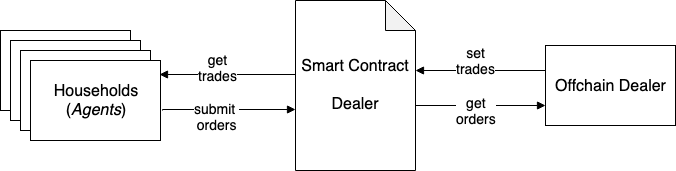
\includegraphics[width=.7\linewidth]{./figures/concept_lem.png}
	\caption{Simplified presentation of the applied communication}
	\label{figure:concept_lem}
\end{figure}

With reference to figure \ref{figure:concept_lem}, the households submit their orders to the dealers' smart contract.  
Afterwards, the dealers' conventional software client, designated as \textit{off-chain} dealer in the figure, fetches all existing orders contained in the smart contract
and solves the \textit{market matching problem}, which is introduced in section \ref{sec:market_clearing_mechanism}.
Secondly, the \textit{off-chain} dealer updates all relevant information in the smart contract, for instance 
the settled orders, the trades, the new market prices and the inventory.
Finally, the households get their respective trades from the dealers' smart contract. 

Anyway, the \textit{off-chain dealer} is necessary due to the complex and costly calculation of the \textit{market matching problem}. 
As mentioned in section \ref{sec:transaction}, each transaction consume gas. Additionally, each mathematical operation in a smart contract
increases the amount of gas to be paid for the respective transaction. As a consequence, implementation and execution of the \textit{market matching problem}
in the smart contract itself would be hard to realize and associated with high transaction costs. 

Hence, a well designed smart contract should move computational complexity \textit{off-chain} 
and focus more on updating state in the contract \shortcite{calculate_cost_eth}. A balance between \textit{on-chain}
and \textit{off-chain} complexity should be found.

In addition, we mentioned in section \ref{sec:btm} that the developed open blockchain-based LEM platform applied a synchronous
call market. That means, the dealer only executes the \textit{market matching problem} after all agents have submitted their orders.
Likewise, we mentioned in section \ref{sec:smart_contract} that smart contracts are only active and run if they called by a transaction.
They will never run on his own or in the background. For this reason, a mechanism is necessary which triggers the execution of the 
\textit{market matching problem}. The implementation of an \textit{off-chain} dealer is also suitable for this.

So far, this section presented the basic idea and concept of the developed open blockchain-based LEM platform
and explained the necessity of all exisiting components. In the following section [ref einfügen!], the setup 
and technical implementation of the simulation will be described in detail. 

However, we stated earlier in this section that the agents of the \textit{BTM} respresent households
and that these households trading bundles of energy resources to minimize the monetary expense. 
In section \ref{sec:btm_problem_overview}, we introduced the individual linear progams of the agents.
Further, we explained in section \ref{sec:agent_bidding} that a rational agent will choose an improving bundle for 
trading which leaves his wealth level on the same level or better off and defined the selection of such a bundle 
as the \textit{bundle determination problem}.
Finally, to embed the \textit{BTM} into the topic of local energy markets, we need to define 
a linear programming problem which depicts the energy efficient demand side management of households.

\subsection{Demand side management of a household}
This subsection will embed the \text{BTM} into the topic of local energy markets. 
Therefore, we will develop a exemplary and simplified linear programming problem in terms of energy efficient demand side management of households.  
That means, the objective of the respective households is to minimize their monetary expense regarding energy consumption.
However, the minimization of the costs due to energy consuming depends on a number of constraints. 
It must be ensured that sufficient energy can be provided at all times.

\shortciteA{Chen2013} developed such a linear programming model for demand side management of households, on which the following
presented model is based. 

First, we introduce all relevant variables. Let $a$ denote an appliance, and $A$ the set of all existing appliances in a household.
In that case, an appliance constitutes energy consuming items, e.g. washers, refrigerators, plug-in hybrid vehicles, etc.
Next, the variable $x_{a}$ denotes the energy consumed by an appliance $a$  to a given point in time. 
Further, each appliance $a \in A$ has a maximum energy level that is defined as rated power and described by $P_{a}$.
Additionally, it exists a limit on the total energy consumed by various appliances of a household. This total 
energy consumption limit is described by $L_{A}$. In case the total energy consumption limit is exceeded, the power network of 
the household will be tripped out.
Moreover, a household consumes on the one hand solar energy from
photovoltaic systems (PV) and on the other hand energy from the electrical grid. 
If households do not consume the solar energy directly, they have the opportunity to 
store it in batteries, or export it back to the main power grid if the battery is full.
Let $e_{g}$ denote the energy used from the electrical grid, and $e_{s}$ the energy produced by the photovoltaic systems.
In addition, let $p_{g}$ and $p_{s}$ denote the unit price of the energy from the electrical grid and solar energy.
Furthermore, we describe the solar energy used by all appliances of a household as $y_{s}$, the consumed battery energy 
as $y_{b}$ and the remaining solar energy which is not used by the household appliances and stored in the battery as $z_{b}$.

Finally, we developed the following linear program for optimization of the household monetary expense.

\begin{equation}
    \begin{array}{ll@{}ll}
        \text{min}  & \displaystyle p_{g} \cdot e_{g} + p_{s} \cdot e_{s} &\\
        \text{s.t.}& \displaystyle \sum\limits_{a \in A}^{} x_{a} \leq L_{A}  \\
					& \displaystyle x_{a} \leq P_{a}, \quad \forall a \in A \\
					& \displaystyle \sum\limits_{a \in A}^{} x_{a} = y_{s} + y_{b} + e_{g} \\
					& \displaystyle y_{s} + z_{b} \leq e_{s}
    \end{array}
\end{equation}

\clearpage
In the table below, all applied variables of the developed linear program are listed:

\begin{longtable}{c|l}
	\hline
    $a$ & energy consuming appliance of household \\
	$A$ & set of all existing energy consuming appliances of household \\
	$x_{a}$ & consumed energy of an appliance $a$ \\
	$P_{a}$ & maximum energy level (rated power) of an appliance $a$ \\
	$L_{A}$ & total energy consumption limit of a household \\
	$e_{g}$ & energy used from the electrical grid \\
	$e_{s}$ & energy produced by PV \\
	$p_{g}$ & unit price of energy from electrical grid \\
	$p_{s}$ & unit price of energy from PV \\
	$y_{s}$ & solar energy used by all appliances of a household \\
	$y_{b}$ & consumed batterie energy by all appliances of a household \\
	$z_{b}$ & remaining unused solar energy stored in the batterie \\
	\hline
	\caption{Applied variables in linear program for optimization of the household monetary expense}
	\label{table:sorted_gas_prices}
\end{longtable} 

As mentioned earlier,
the objective of the respective households is to minimize
their monetary expense regarding energy consumption.
The term $p_{g} \cdot e_{g}$ denotes the costs for energy from the electrical
grid, whereas the term $p_{s} \cdot e_{s}$ denotes the costs for energy from photovoltaic systems. 

Besides, the first constraint ensures that the total energy consumption of all energy consuming
appliances of a household not exceeds the limit $L_{A}$. 

Next, the second constraint describes the requirement that the consumed energy
for all existing appliances $a$ in a household is less or equal 
to the respective rated power $P_{a}$.

Further, the third constraint makes sure that the energy consumed by all appliances
of a household is the sum of the energy from the electrical grid, the solar energy from 
the PV system and the battery energy. This implies, if the amount of solar and battery 
energy is not sufficient to cover the energy consumption of all appliances, external 
energy from the electrical grid will be used. Therefore, it is ensured 
that sufficient energy is available at all times.

Finally, the fourth constraint describes that the solar energy produced by the PV system 
is greater or equal to the sum of the consumed and stored solar energy. 
At times when the battery is fully charged and the energy consumption of the 
appliances is covered by solar energy, it is possible to sell the surplus of 
wasted solar energy.
Referring to the \textit{BTM}, the first two constraints of the proposed linear
programming model constitute the independent resources that are managed locally.
The shared resources are represented by 
the energy resources $e_{g}$ and $e_{s}$.
Therefore the respective households trade the following limited bundles.

\begin{equation*}
    \begin{array}{ll@{}ll}
		w = 
		\begin{pmatrix}
			e_{g} \\
			e_{s}
		\end{pmatrix}
    \end{array}
\end{equation*}

Consequently, the objective of the linear programming 
model written in matrix-vector notation.

\begin{equation*}
    \begin{array}{ll@{}ll}
		\text{min}  & \displaystyle p^{T} \cdot w
    \end{array}
\end{equation*}

where $p^{T}$ denotes the transposed price vector.

\begin{equation*}
    \begin{array}{ll@{}ll}
		p^{T} = 
		\begin{pmatrix}
			p_{g} &
			p_{s}
		\end{pmatrix}
    \end{array}
\end{equation*}


To sum up, this subsection presented a simplified linear 
programming model for demand side management of a household
that can be integrated into the proposed \textit{BTM}.

Furthmore, the developed model should only serve as an inspiration and example
and has no claim to completeness. 
It is intended to illustrate how the presented framework can be adapted to enable the trading 
of energy resourcres in a local energy market. 
Thus, researchers without a deep technically background are able to use this platform and
develop and investigate their concepts 

Finally, the following section will present the implementation of the developed platform in depth.

\clearpage